% http://en.wikibooks.org/wiki/LaTeX/Title_Creation
% Adjusted for EPFL template


\begin{titlepage}


\vspace{3\baselineskip}

\raisebox{3cm}[1.5cm]{
\hspace{-4cm}
\def\arraystretch{1.5}
{\scriptsize
\begin{tabular} {p{4.1cm}m{5cm}p{2cm}m{4.6cm}}
 
\rule{0pt}{1cm}    
\multirow{3}{*}{\raisebox{\totalheight}{
\includegraphics[height=0.15\columnwidth]{epfl}}} & \textbf{School of Computer and Communication Sciences}  &
\multirow{3}{*}{
\includegraphics[height=0.15	\columnwidth]{cern.jpg}} & \textbf{Information and Technology Department}\\ 

& Computer Science Section & &Digital Library Service \\
& Distributed Information System Laboratory (LSIR) &&  \\ \\ \hline
\end{tabular}
}
}

\begin{center}


\vspace{1cm}
\newcommand{\HRule}{\rule{\linewidth}{0.3mm}}


    {\LARGE \bfseries  $5e^{x+y}$: A Math Aware Search Engine (for CDS)} \\
	\vspace{1cm}    
    \textsc{\Large Master Thesis Project} \\
    
	
	\vspace{3mm}
	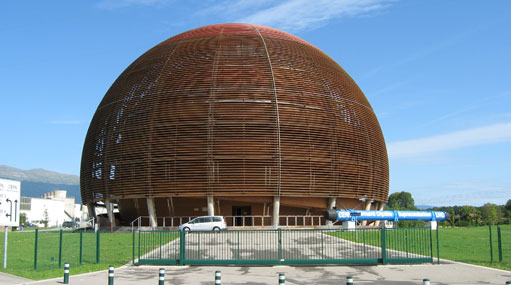
\includegraphics[height=6 cm]{cern_logo1.jpg}
	\vspace{1cm}
	\HRule 
	
	\emph{Author:} \\Arthur \textsc{Oviedo}\\
    \vspace{1cm}

    \emph{Supervisors:} \\   
    CERN: Nikolaos \textsc{Kasioumis} \\   
    EPFL: Karl \textsc{Aberer}\\
    
    % Bottom of the page
	\vfill
	{\large \today}


\end{center}

\end{titlepage}

